\documentclass[multi=tikzpicture,border=8pt]{standalone}
\usepackage[UTF8]{ctex}
\usepackage{amsmath,amssymb,tikz}
\usetikzlibrary{arrows.meta,calc}
\definecolor{blue}{HTML}{17365D}
\definecolor{red}{HTML}{AC3931}
\tikzset{every node/.style={font=\small},arrow/.style={-{Stealth[length=2.8mm]},thick},dim/.style={|<->|,thin},box/.style={draw,rounded corners,align=center,minimum width=2.5cm,minimum height=.8cm}}
\begin{document}
\begin{tikzpicture}
\draw[blue,very thick](0,0)circle(2);\fill[red](2,0)circle(4pt)node[right]{电子};\draw[arrow,blue](2,.15)--(2,1.3)node[right]{$v$};\foreach \x/\y in {-1/0,0/0,1/0,0/1,0/-1}{\draw(\x,\y)circle(.09);\fill(\x,\y)circle(1pt);}\node[above]at(0,2.4){$B>0,\ \dot B>0$};\draw[arrow,red](1.8,0)--(.8,0)node[below,midway]{$F_B$};\draw[arrow,red](2,-.1)--(2,-1.2)node[right]{$E_\varphi$};
\end{tikzpicture}
\begin{tikzpicture}
\draw[blue,very thick](0,0)circle(2);\fill[red](2,0)circle(4pt)node[right]{电子};\draw[arrow,blue](2,.15)--(2,1.3)node[right]{$v$};\foreach \x/\y in {-1/0,0/0,1/0,0/1,0/-1}{\draw(\x,\y)circle(.09);\fill(\x,\y)circle(1pt);}\node[above]at(0,2.4){$B>0,\ \dot B>0$};\draw[arrow,red](2.6,0)--(2.6,1.2)node[right]{$-e\boldsymbol E$};\draw[arrow,red](-2,.8)--(-2,-.7)node[left]{电子加速};\node[below]at(0,-2.5){$E_\varphi=-r\dot B/2$};
\end{tikzpicture}
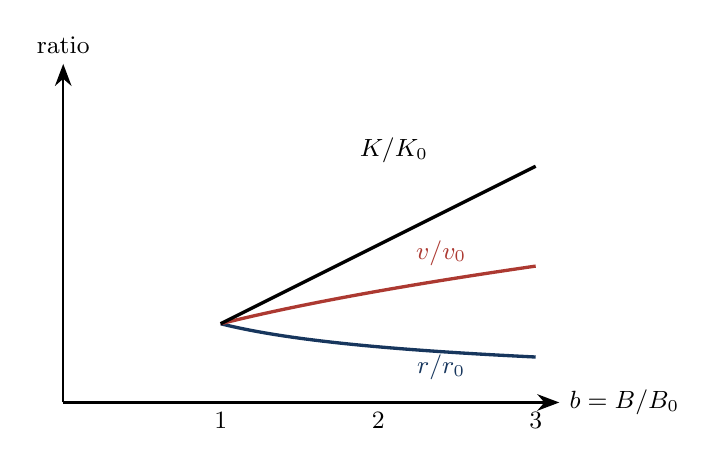
\begin{tikzpicture}
\draw[arrow](0,0)--(6.3,0)node[right]{$b=B/B_0$};\draw[arrow](0,0)--(0,4.3)node[above]{$\mathrm{ratio}$};\draw[very thick,blue] plot coordinates {(2.00000,1.00000) (2.04040,0.99005) (2.08081,0.98039) (2.12121,0.97101) (2.16162,0.96189) (2.20202,0.95303) (2.24242,0.94440) (2.28283,0.93601) (2.32323,0.92783) (2.36364,0.91987) (2.40404,0.91210) (2.44444,0.90453) (2.48485,0.89715) (2.52525,0.88994) (2.56566,0.88291) (2.60606,0.87604) (2.64646,0.86932) (2.68687,0.86276) (2.72727,0.85635) (2.76768,0.85008) (2.80808,0.84394) (2.84848,0.83793) (2.88889,0.83205) (2.92929,0.82629) (2.96970,0.82065) (3.01010,0.81513) (3.05051,0.80971) (3.09091,0.80440) (3.13131,0.79919) (3.17172,0.79409) (3.21212,0.78908) (3.25253,0.78416) (3.29293,0.77933) (3.33333,0.77460) (3.37374,0.76994) (3.41414,0.76537) (3.45455,0.76089) (3.49495,0.75647) (3.53535,0.75214) (3.57576,0.74788) (3.61616,0.74369) (3.65657,0.73957) (3.69697,0.73552) (3.73737,0.73153) (3.77778,0.72761) (3.81818,0.72375) (3.85859,0.71995) (3.89899,0.71621) (3.93939,0.71253) (3.97980,0.70890) (4.02020,0.70533) (4.06061,0.70181) (4.10101,0.69834) (4.14141,0.69493) (4.18182,0.69156) (4.22222,0.68825) (4.26263,0.68498) (4.30303,0.68175) (4.34343,0.67858) (4.38384,0.67544) (4.42424,0.67235) (4.46465,0.66930) (4.50505,0.66629) (4.54545,0.66332) (4.58586,0.66040) (4.62626,0.65751) (4.66667,0.65465) (4.70707,0.65184) (4.74747,0.64906) (4.78788,0.64631) (4.82828,0.64360) (4.86869,0.64093) (4.90909,0.63828) (4.94949,0.63567) (4.98990,0.63310) (5.03030,0.63055) (5.07071,0.62803) (5.11111,0.62554) (5.15152,0.62309) (5.19192,0.62066) (5.23232,0.61826) (5.27273,0.61588) (5.31313,0.61354) (5.35354,0.61122) (5.39394,0.60892) (5.43434,0.60665) (5.47475,0.60441) (5.51515,0.60219) (5.55556,0.60000) (5.59596,0.59783) (5.63636,0.59568) (5.67677,0.59356) (5.71717,0.59146) (5.75758,0.58938) (5.79798,0.58732) (5.83838,0.58529) (5.87879,0.58327) (5.91919,0.58128) (5.95960,0.57930) (6.00000,0.57735)};\draw[very thick,red] plot coordinates {(2.00000,1.00000) (2.04040,1.01005) (2.08081,1.02000) (2.12121,1.02986) (2.16162,1.03962) (2.20202,1.04929) (2.24242,1.05887) (2.28283,1.06837) (2.32323,1.07778) (2.36364,1.08711) (2.40404,1.09637) (2.44444,1.10554) (2.48485,1.11464) (2.52525,1.12367) (2.56566,1.13262) (2.60606,1.14150) (2.64646,1.15032) (2.68687,1.15907) (2.72727,1.16775) (2.76768,1.17637) (2.80808,1.18492) (2.84848,1.19342) (2.88889,1.20185) (2.92929,1.21023) (2.96970,1.21854) (3.01010,1.22680) (3.05051,1.23501) (3.09091,1.24316) (3.13131,1.25126) (3.17172,1.25931) (3.21212,1.26730) (3.25253,1.27525) (3.29293,1.28315) (3.33333,1.29099) (3.37374,1.29880) (3.41414,1.30655) (3.45455,1.31426) (3.49495,1.32192) (3.53535,1.32954) (3.57576,1.33712) (3.61616,1.34465) (3.65657,1.35214) (3.69697,1.35959) (3.73737,1.36700) (3.77778,1.37437) (3.81818,1.38170) (3.85859,1.38899) (3.89899,1.39624) (3.93939,1.40346) (3.97980,1.41064) (4.02020,1.41778) (4.06061,1.42489) (4.10101,1.43196) (4.14141,1.43900) (4.18182,1.44600) (4.22222,1.45297) (4.26263,1.45990) (4.30303,1.46680) (4.34343,1.47367) (4.38384,1.48051) (4.42424,1.48732) (4.46465,1.49410) (4.50505,1.50084) (4.54545,1.50756) (4.58586,1.51424) (4.62626,1.52090) (4.66667,1.52753) (4.70707,1.53412) (4.74747,1.54069) (4.78788,1.54724) (4.82828,1.55375) (4.86869,1.56024) (4.90909,1.56670) (4.94949,1.57313) (4.98990,1.57954) (5.03030,1.58592) (5.07071,1.59228) (5.11111,1.59861) (5.15152,1.60492) (5.19192,1.61120) (5.23232,1.61746) (5.27273,1.62369) (5.31313,1.62990) (5.35354,1.63608) (5.39394,1.64225) (5.43434,1.64838) (5.47475,1.65450) (5.51515,1.66060) (5.55556,1.66667) (5.59596,1.67272) (5.63636,1.67874) (5.67677,1.68475) (5.71717,1.69074) (5.75758,1.69670) (5.79798,1.70264) (5.83838,1.70856) (5.87879,1.71447) (5.91919,1.72035) (5.95960,1.72621) (6.00000,1.73205)};\draw[very thick,black] plot coordinates {(2.00000,1.00000) (2.04040,1.02020) (2.08081,1.04040) (2.12121,1.06061) (2.16162,1.08081) (2.20202,1.10101) (2.24242,1.12121) (2.28283,1.14141) (2.32323,1.16162) (2.36364,1.18182) (2.40404,1.20202) (2.44444,1.22222) (2.48485,1.24242) (2.52525,1.26263) (2.56566,1.28283) (2.60606,1.30303) (2.64646,1.32323) (2.68687,1.34343) (2.72727,1.36364) (2.76768,1.38384) (2.80808,1.40404) (2.84848,1.42424) (2.88889,1.44444) (2.92929,1.46465) (2.96970,1.48485) (3.01010,1.50505) (3.05051,1.52525) (3.09091,1.54545) (3.13131,1.56566) (3.17172,1.58586) (3.21212,1.60606) (3.25253,1.62626) (3.29293,1.64646) (3.33333,1.66667) (3.37374,1.68687) (3.41414,1.70707) (3.45455,1.72727) (3.49495,1.74747) (3.53535,1.76768) (3.57576,1.78788) (3.61616,1.80808) (3.65657,1.82828) (3.69697,1.84848) (3.73737,1.86869) (3.77778,1.88889) (3.81818,1.90909) (3.85859,1.92929) (3.89899,1.94949) (3.93939,1.96970) (3.97980,1.98990) (4.02020,2.01010) (4.06061,2.03030) (4.10101,2.05051) (4.14141,2.07071) (4.18182,2.09091) (4.22222,2.11111) (4.26263,2.13131) (4.30303,2.15152) (4.34343,2.17172) (4.38384,2.19192) (4.42424,2.21212) (4.46465,2.23232) (4.50505,2.25253) (4.54545,2.27273) (4.58586,2.29293) (4.62626,2.31313) (4.66667,2.33333) (4.70707,2.35354) (4.74747,2.37374) (4.78788,2.39394) (4.82828,2.41414) (4.86869,2.43434) (4.90909,2.45455) (4.94949,2.47475) (4.98990,2.49495) (5.03030,2.51515) (5.07071,2.53535) (5.11111,2.55556) (5.15152,2.57576) (5.19192,2.59596) (5.23232,2.61616) (5.27273,2.63636) (5.31313,2.65657) (5.35354,2.67677) (5.39394,2.69697) (5.43434,2.71717) (5.47475,2.73737) (5.51515,2.75758) (5.55556,2.77778) (5.59596,2.79798) (5.63636,2.81818) (5.67677,2.83838) (5.71717,2.85859) (5.75758,2.87879) (5.79798,2.89899) (5.83838,2.91919) (5.87879,2.93939) (5.91919,2.95960) (5.95960,2.97980) (6.00000,3.00000)};\node[blue]at(4.8,.45){$r/r_0$};\node[red]at(4.8,1.9){$v/v_0$};\node at(4.2,3.2){$K/K_0$};\node[below]at(2,0){1};\node[below]at(4,0){2};\node[below]at(6,0){3};
\end{tikzpicture}
\begin{tikzpicture}

\draw[gray,dashed](0,0)circle(2);\draw[blue,very thick](0,0)circle(1.414);\draw[red,very thick](.5,0)circle(1.5);\fill(0,0)circle(2pt)node[below left]{旧中心};\fill[red](.5,0)circle(2pt)node[below right]{新中心};\node[blue]at(-2.4,1.5){慢变$r_0/\sqrt2$};\node[red]at(2.8,1.5){骤变$3r_0/4$};\node[below]at(0,-2.6){同样加倍，轨道条件不同};

\end{tikzpicture}
\begin{tikzpicture}

\node[box,fill=blue!8](a)at(0,0){慢变近圆\\$K_f=2K_0$};\node[box,fill=red!8](b)at(4.5,0){骤变偏心\\$K_+=9K_0/4$};\node[box](c)at(2.2,-2){完整正则角动量守恒};\draw[arrow](c)--(a);\draw[arrow](c)--(b);\node[above]at(2.2,1.4){$B_f=2B_0$};

\end{tikzpicture}
\end{document}
